% !TEX program = xelatex
% 第二讲：处理 p(x) 的五种方式
\documentclass[aspectratio=169,10pt,UTF8,fontset=none]{ctexbeamer}
% Preamble for this offering's decks.
% Lookup order for \input and figures: this folder, then ../shared/ (theme and
% slide-only figures), then ../../figures/ (the book's figures). `make slides`
% sets TEXINPUTS accordingly; \input@path covers compiling directly in this folder.
\makeatletter
\def\input@path{{../shared/}}
\makeatother
\usepackage{beamerthemegenai}
\graphicspath{{figures/}{../shared/figures/}{../../figures/}}

\title{生成模型与概率统计}
\author{张士欣}
\institute{中国科学院物理研究所}
\date{2026.10}
\renewcommand{\titlefigure}{cover_probability_flow.pdf}
\renewcommand*{\titleurl}{github.com/refraction-ray/free-energy-to-llms}

\subtitle{第二讲\quad 处理 $p(x)$ 的五种方式}
\renewcommand{\lecturename}{第二讲\quad 处理 $p(x)$ 的五种方式}

\begin{document}

\begin{frame}[plain]
  \titlepage
\end{frame}

\begin{frame}{上一讲留下的问题}
  \begin{columns}[T]
    \begin{column}{0.48\textwidth}
      \begin{itemize}
        \item 训练目标：极大似然 $=$ 最小化 $\KL(\hat\pi\Vert p_\theta)$，需要能逐点计算 $\log p_\theta(x)$
        \item 从能量出发：最小化 $\KL(q\Vert\pi)$，即变分自由能
        \item 难点：高维分布的归一化常数 $Z$；不知道 $Z$，既算不出密度，也不能直接抽样
      \end{itemize}
      \vspace{2mm}
      本讲沿地图依次看五类模型怎样处理 $p(x)$，每一类都回答同样四个问题。
    \end{column}
    \begin{column}{0.5\textwidth}
      \centering
      \fourstack{密度、条件概率、能量，还是密度的梯度？}{优化哪个散度或下界？}{一次前向、逐步生成、微分方程，还是马尔可夫链？}{成本与失效模式在哪里？}
    \end{column}
  \end{columns}
\end{frame}

\begin{frame}{本讲路线}
  \centering
  \input{figures/genmap.tex}
  \vfill
  {\small 本讲：自回归、Flow、VAE、GAN、能量模型；扩散留到第三讲。}
\end{frame}

% ====================================================================
\section{自回归：把联合分布拆开}

\begin{frame}{链式法则}
  \begin{columns}[T]
    \begin{column}{0.5\textwidth}
      对序列 $x=(x_1,\ldots,x_T)$，恒有
      \setlength{\abovedisplayskip}{5pt}\setlength{\belowdisplayskip}{5pt}%
      \[
        p(x)=\textstyle\prod_{t=1}^{T}p(x_t\mid x_{<t})
      \]
      \begin{itemize}
        \item 直接给每个序列赋概率要 $|\mathcal V|^T$ 个数；$|\mathcal V|=10^5$、$T=1000$ 时是 $10^{5000}$
        \item 分解后每一步只需一个 $|\mathcal V|$ 类的 categorical 分布，由同一个网络读入前缀给出
        \item 每个因子都已归一化，乘积自动归一化：$Z=1$
      \end{itemize}
      \begin{concept}{链式法则}
        恒等式，不含近似；近似只在用网络表示条件分布这一步。
      \end{concept}
    \end{column}
    \begin{column}{0.47\textwidth}
      \centering
      \begin{tikzpicture}[x=1mm,y=1mm]
        \node[nsoft] (r) at (0,20) {BOS};
        \node[nteal] (a) at (20,34) {猫};
        \node[nsoft] (b) at (20,20) {狗};
        \node[nsoft] (c) at (20,6) {鸟};
        \draw[arteal,line width=1pt] (r) -- node[lblt,above,sloped] {0.5} (a);
        \draw[ar] (r) -- node[lbl,above] {0.3} (b);
        \draw[ar] (r) -- node[lbl,below,sloped] {0.2} (c);
        \node[nteal] (a1) at (42,42) {坐};
        \node[nsoft] (a2) at (42,30) {跑};
        \draw[arteal,line width=1pt] (a) -- node[lblt,above,sloped] {0.6} (a1);
        \draw[ar] (a) -- node[lbl,below,sloped] {0.4} (a2);
        \node[lbl] at (42,18) {$\vdots$};
        \node[lbl] at (42,6) {$\vdots$};
        \node[lblt,anchor=north] at (24,-2) {$p(\text{猫},\text{坐})=0.5\times0.6=0.3$};
      \end{tikzpicture}
      \par
      {\small 顺序同时规定了采样程序：沿树从根走到叶。图像也可以排成序列，从左到右、从上到下逐个生成：早期逐像素；现在多先压成离散 token 网格，一个 token 对应一小块区域。}
    \end{column}
  \end{columns}
\end{frame}

\begin{frame}{从极大似然到逐 token 交叉熵}
  \begin{keystep}
    把链式分解代入第一讲的 MLE：
    \keyeq{
      -\frac1N\sum_{i}\log p_\theta(x^{(i)})
      =-\frac1N\sum_i\sum_{t}\log p_\theta\bigl(x^{(i)}_t\mid x^{(i)}_{<t}\bigr)
      =\frac1N\sum_i\sum_t\mathrm{CE}\bigl(e_{x^{(i)}_t},\,\pi_{\theta,t}\bigr)}
    其中 $\pi_{\theta,t}$ 是网络在位置 $t$ 输出的词表分布，$e_{x_t}$ 是真实 token 的 one-hot 向量。
  \end{keystep}
  \begin{columns}[T]
    \begin{column}{0.5\textwidth}
      \begin{itemize}
        \item 每个位置都是一道 $|\mathcal V|$ 类的分类题，标签是真实的下一个 token
        \item 一条序列提供 $T$ 道题，全部无须人工标注
      \end{itemize}
    \end{column}
    \begin{column}{0.47\textwidth}
      \begin{takeaway}
        大语言模型的预训练损失，就是这个分解下的极大似然。
      \end{takeaway}
    \end{column}
  \end{columns}
\end{frame}

\begin{frame}{训练并行，生成串行}
  \centering
  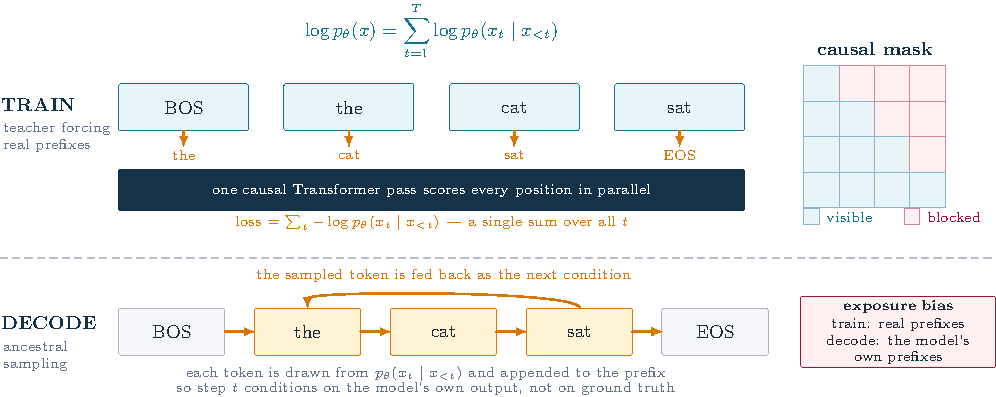
\includegraphics[width=0.95\textwidth]{autoregressive_train_decode.pdf}
  \vfill
  \begin{columns}[T]
    \begin{column}{0.48\textwidth}
      \small
      \textbf{Teacher forcing}：训练时每个位置都读真实前缀；因果 mask 让所有位置在一次前向中并行计算。
    \end{column}
    \begin{column}{0.48\textwidth}
      \small
      \textbf{Ancestral sampling}：生成时抽到的 token 要放回条件里，必须一个一个来。训练见真实前缀、部署见自己的前缀，这个差异叫 exposure bias。
    \end{column}
  \end{columns}
\end{frame}

\begin{frame}{采样温度与截断}
  \begin{columns}[c]
    \begin{column}{0.56\textwidth}
      \centering
      \begin{tikzpicture}[x=1mm,y=1mm]
        \foreach \g/\tv/\vals in {0/0.5/{0.688,0.170,0.076,0.042,0.019,0.006},1/1/{0.429,0.213,0.143,0.106,0.071,0.039},2/2/{0.287,0.202,0.166,0.142,0.117,0.086}}{%
          \begin{scope}[shift={(\g*27,0)}]
            \foreach \p [count=\i from 0] in \vals {\fill[GTeal!80] (\i*3.6,6) rectangle ++(2.8,\p*40);}
            \draw[GSlate!60] (-0.5,6) -- (21.5,6);
            \node[lbl] at (10.5,2) {$\tau=\tv$};
          \end{scope}}
      \end{tikzpicture}
      \par\vspace{1mm}
      {\scriptsize\slate{同一组 logit（“好、热、冷、不错、晴朗、糟”）在三种温度下的分布}}
    \end{column}
    \begin{column}{0.42\textwidth}
      \[
        p_\tau(v)=\frac{e^{l_v/\tau}}{\sum_u e^{l_u/\tau}}
      \]
      \begin{itemize}
        \item $\tau<1$ 更尖，$\tau>1$ 更平
        \item top-$k$ / top-$p$：只保留概率最高的一部分 token，再重新归一化
        \item 只有 $\tau=1$ 且不截断时，抽样才严格服从模型自身的分布
      \end{itemize}
      \begin{concept}{玻尔兹曼分布}
        softmax 就是以 $-l_v$ 为能量、$\tau$ 为温度的玻尔兹曼分布。
      \end{concept}
    \end{column}
  \end{columns}
\end{frame}

\begin{frame}{自回归：小结}
  \centering
  \fourcard%
    {$p_\theta(x)=\prod_t p_\theta(x_t\mid x_{<t})$\\显式、精确归一化}%
    {逐 token 交叉熵\\$=$ 极大似然}%
    {从左到右逐个抽样\\温度、top-$k$、top-$p$}%
    {生成串行，延迟随长度增长；exposure bias}
  \vfill
  \begin{takeaway}
    自回归是离散序列的首选：似然精确、训练稳定、条件可以随时改变。对连续数据（图像、坐标）没有天然的“下一个”，串行生成也慢，于是需要别的路线。
  \end{takeaway}
\end{frame}

% ====================================================================
\section{Normalizing Flow：可逆变换}

\begin{frame}{变量替换：概率质量守恒}
  \begin{columns}[c]
    \begin{column}{0.55\textwidth}
      \centering
      \begin{tikzpicture}
        \begin{axis}[genai,name=base,width=4.4cm,height=3.8cm,xmin=-3.5,xmax=3.5,ymin=0,ymax=0.45,xtick=\empty,ytick=\empty,xlabel={$z$},domain=-3.5:3.5,title={\scriptsize $p_Z=\mathcal N(0,1)$},title style={yshift=-1ex}]
          \addplot[GSlate,fill=GSlate!15] {exp(-x^2/2)/sqrt(2*pi)} \closedcycle;
        \end{axis}
        \begin{axis}[genai,at={(base.east)},anchor=west,xshift=1.4cm,width=4.4cm,height=3.8cm,xmin=-4.3,xmax=4.3,ymin=0,ymax=0.45,xtick=\empty,ytick=\empty,xlabel={$x$},title={\scriptsize $p_X$},title style={yshift=-1ex}]
          \addplot[GTeal,fill=GSky,domain=-3.5:3.5,samples=241,variable=\t] ({\t+0.8*tanh(2*\t)},{exp(-\t^2/2)/sqrt(2*pi)/(1+1.6/cosh(2*\t)^2)}) \closedcycle;
        \end{axis}
        \draw[ar,line width=1pt] ([xshift=1mm]base.east) -- node[lbl,above] {$x=g(z)$} ++(1.2cm,0);
      \end{tikzpicture}
      \par\vspace{1mm}
      {\scriptsize\slate{$g(z)=z+0.8\tanh 2z$：中间被拉伸，密度变低；两侧被压缩，密度升高}}
    \end{column}
    \begin{column}{0.43\textwidth}
      一维单调变换 $x=g(z)$ 下，小区间里的概率不变：
      \[
        p_X(x)\,|dx|=p_Z(z)\,|dz|
      \]
      \[
        \Rightarrow\ p_X(x)=p_Z\bigl(g^{-1}(x)\bigr)\left|\frac{dg^{-1}}{dx}\right|
      \]
      \begin{concept}{随机变量函数的密度}
        这是概率课里的变换公式；Flow 把它当作建模工具：选一个简单的 $p_Z$，学一个可逆的 $g$。
      \end{concept}
    \end{column}
  \end{columns}
\end{frame}

\begin{frame}{高维：Jacobian 行列式记录体积变化}
  \begin{columns}[c]
    \begin{column}{0.5\textwidth}
      令 $z=f_\theta(x)$ 可逆可微，
      \[
        \log p_X(x)=\log p_Z\bigl(f_\theta(x)\bigr)+\log\left|\det\frac{\partial f_\theta}{\partial x}\right|
      \]
      \begin{itemize}
        \item 训练：极大似然，直接用上式
        \item 采样：$z\sim\mathcal N(0,I)$，再算 $x=f_\theta^{-1}(z)$
      \end{itemize}
      \begin{caution}[两个障碍]任意网络不一定可逆；$d\times d$ 行列式要 $O(d^3)$，图像的 $d\sim10^5$。\end{caution}
    \end{column}
    \begin{column}{0.47\textwidth}
      \centering
      \begin{tikzpicture}[x=1mm,y=1mm]
        \foreach \u in {0,4,...,20}{\draw[GSlate!45] (\u,0) -- (\u,20); \draw[GSlate!45] (0,\u) -- (20,\u);}
        \fill[GTeal!35] (8,8) rectangle (12,12);
        \node[lbl,anchor=north] at (10,-1) {$x$ 空间};
        \draw[ar,line width=1pt] (23,10) -- node[lbl,above] {$f_\theta$} (31,10);
        \begin{scope}[shift={(34,0)}]
          \foreach \u in {0,4,...,20}{%
            \draw[GSlate!45] plot[domain=0:20,samples=20] ({\u+1.5*sin(\x*9)},{\x+0.02*\u*\u});
            \draw[GSlate!45] plot[domain=0:20,samples=20] ({\x+1.5*sin(\u*9)},{\u+0.02*\x*\x});}
          \fill[GOrange!45] plot[domain=8:12,samples=6] ({\x+1.5*sin(8*9)},{8+0.02*\x*\x}) --
            plot[domain=8:12,samples=6] ({12+1.5*sin(\x*9)},{\x+0.02*144}) --
            plot[domain=12:8,samples=6] ({\x+1.5*sin(12*9)},{12+0.02*\x*\x}) --
            plot[domain=12:8,samples=6] ({8+1.5*sin(\x*9)},{\x+0.02*64}) -- cycle;
          \node[lbl,anchor=north] at (11,-1) {$z$ 空间};
        \end{scope}
        \node[lblo,anchor=north] at (30,-7) {小方格的面积比 $=|\det J|$};
      \end{tikzpicture}
    \end{column}
  \end{columns}
\end{frame}

\begin{frame}{Coupling layer：让 Jacobian 变成三角阵}
  \centering
  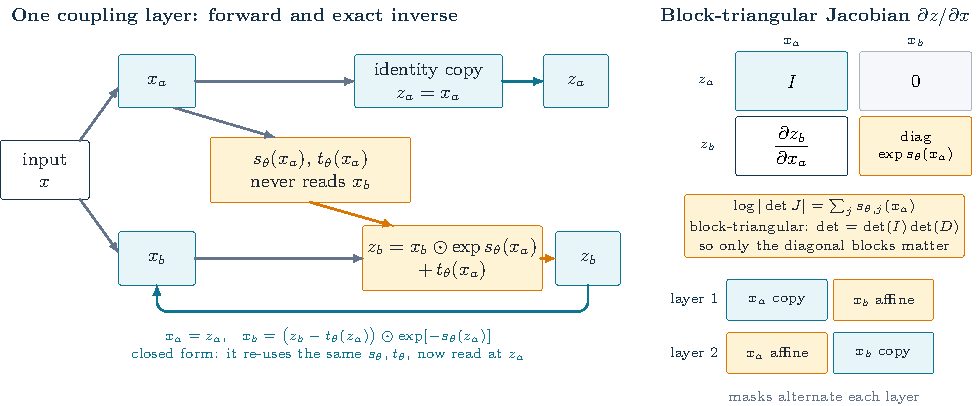
\includegraphics[width=0.95\textwidth]{realnvp_architecture.pdf}
  \vfill
  \begin{columns}[T]
    \begin{column}{0.5\textwidth}
      \small
      $z_a=x_a$，$z_b=x_b\odot e^{s_\theta(x_a)}+t_\theta(x_a)$。$s_\theta,t_\theta$ 可以是任意网络，它们本身不必可逆。
    \end{column}
    \begin{column}{0.47\textwidth}
      \small
      块三角 Jacobian：$\log|\det J|=\sum_js_{\theta,j}(x_a)$，代价从 $O(d^3)$ 降到 $O(d)$；相邻层交换 $a,b$ 的划分。
    \end{column}
  \end{columns}
\end{frame}

\begin{frame}{连续极限：沿速度场搬运概率}
  \begin{columns}[c]
    \begin{column}{0.5\textwidth}
      \centering
      \begin{tikzpicture}[x=1mm,y=1mm]
        \draw[GSlate!50] (0,0) -- (0,40);
        \draw[GSlate!50] (50,0) -- (50,40);
        \fill[GSlate!20] plot[domain=0:40,samples=60] ({-7*exp(-(\x-20)^2/72)},\x) -- (0,40) -- (0,0) -- cycle;
        \fill[GSky] plot[domain=0:40,samples=80] ({50+6*exp(-(\x-8)^2/6)+6*exp(-(\x-32)^2/6)},\x) -- (50,40) -- (50,0) -- cycle;
        \foreach \s/\e in {8/5,12/6.5,15/8,18/9.5,19.5/11,20.5/29,22/30.5,25/32,28/33.5,32/35}{%
          \draw[GTeal,line width=0.7pt] (0,\s) .. controls (20,\s) and (30,\e) .. (50,\e);}
        \node[lbl,anchor=north] at (0,-1) {$r=0$：$\mathcal N(0,1)$};
        \node[lbl,anchor=north] at (50,-1) {$r=1$：数据};
        \node[lblt,anchor=south] at (25,40) {$dx/dr=v_\theta(x,r)$};
      \end{tikzpicture}
    \end{column}
    \begin{column}{0.48\textwidth}
      把 $x_{k+1}=x_k+\Delta r\,v_\theta(x_k,r_k)$ 取 $\Delta r\to0$：
      \[
        \frac{dx}{dr}=v_\theta(x,r),\qquad
        \frac{d\log p_r(x_r)}{dr}=-\nabla\cdot v_\theta
      \]
      \begin{itemize}
        \item 速度网络可以自由设计，不再需要特殊结构
        \item 代价：极大似然训练时，每个样本都要解一次 ODE、沿轨迹积分散度，再让梯度穿过整个求解过程
      \end{itemize}
      \begin{concept}{连续性方程}
        $\partial_rp_r+\nabla\cdot(p_rv)=0$：概率像流体一样被搬运，总量守恒。第三讲的 Flow Matching 保留这个模型，换掉的是训练方式。
      \end{concept}
    \end{column}
  \end{columns}
\end{frame}

\begin{frame}{Flow：小结}
  \centering
  \fourcard%
    {可逆映射 $x=f_\theta^{-1}(z)$\\变量替换给出精确密度}%
    {精确负对数似然\\$-\log p_Z(f(x))-\log|\det J|$}%
    {$z\sim\mathcal N(0,I)$ 后运行逆变换\\一次前向}%
    {可逆性限制网络结构；高维时样本质量常不如扩散}
  \vfill
  \begin{takeaway}
    Flow 同时给出精确似然、可逆编码和直接采样，代价是网络必须同维且可逆。如果允许潜变量维度低于数据、映射不可逆，就得放弃精确似然，这就是 VAE。
  \end{takeaway}
\end{frame}

% ====================================================================
\section{VAE：隐变量与变分下界}

\begin{frame}{隐变量：观测背后的低维原因}
  \begin{columns}[T]
    \begin{column}{0.5\textwidth}
      人脸由姿态、光照、表情等少数因素决定。先抽因素，再生成观测：
      \[
        p_\theta(x)=\int p(z)\,p_\theta(x\mid z)\,dz,\quad p(z)=\mathcal N(0,I)
      \]
      \begin{itemize}
        \item decoder 读入 $z$，输出 $p_\theta(x\mid z)$ 的参数
        \item 非线性 decoder 下积分没有解析解，后验 $p_\theta(z\mid x)$ 同样难算
      \end{itemize}
      \begin{concept}{边缘化与混合分布}
        每个 $z$ 给出一个分量 $p_\theta(x\mid z)$，$p_\theta(x)$ 是所有分量按 $p(z)$ 加权的叠加。分量有无穷多个，$\log p_\theta(x)$ 无法逐点算出，下一页用 ELBO 绕开。
      \end{concept}
    \end{column}
    \begin{column}{0.47\textwidth}
      \centering
      \begin{tikzpicture}[x=1mm,y=1mm]
        \foreach \r/\o in {3/0.9,6/0.6,9/0.35}{\draw[GTeal,opacity=\o] (10,15) circle (\r);}
        \fill[GOrange] (13,17) circle (0.9);
        \node[lbl,anchor=north] at (10,3) {$z\sim\mathcal N(0,I)$};
        \draw[ar,line width=1pt] (22,15) -- node[lbl,above] {decoder} (32,15);
        \draw[GSky,line width=5mm,line cap=round] plot[smooth] coordinates {(36,4) (42,20) (50,10) (58,26)};
        \draw[GTeal,line width=0.8pt] plot[smooth] coordinates {(36,4) (42,20) (50,10) (58,26)};
        \fill[GOrange] (46.6,14.6) circle (0.9);
        \draw[GOrange,dashed] (46.6,14.6) circle (2.6);
        \node[lbl,anchor=north] at (47,3) {$x$ 空间中的弯曲流形};
        \node[lblo,anchor=west] at (34,25) {$p_\theta(x\mid z)$};
      \end{tikzpicture}
      \par\vspace{1mm}
      {\scriptsize\slate{一个 $z$ 对应一个小高斯（虚线圈）；所有 $z$ 的小高斯叠在一起，就是浅蓝色的 $p_\theta(x)$}}
    \end{column}
  \end{columns}
\end{frame}

\begin{frame}{ELBO：把难算的对数似然换成下界}
  \begin{columns}[T]
    \begin{column}{0.62\textwidth}
      引入 encoder $q_\phi(z\mid x)$ 近似后验：
      \begin{keystep}
        \keyeq{
          \log p_\theta(x)&=\underbrace{\E_{q_\phi}\bigl[\log p_\theta(x\mid z)\bigr]-\KL\bigl(q_\phi(z\mid x)\Vert p(z)\bigr)}_{\mathrm{ELBO}}\\
          &\quad+\KL\bigl(q_\phi(z\mid x)\Vert p_\theta(z\mid x)\bigr)}
        把贝叶斯公式 $p_\theta(z\mid x)=p_\theta(x,z)/p_\theta(x)$ 代入最后一项即可验证。
      \end{keystep}
      \begin{itemize}
        \item 第一项：重构，已观测的 $x$ 在 decoder 分布下的对数概率
        \item 第二项：编码分布不要偏离先验，否则从先验采样会落到没训练过的区域
      \end{itemize}
    \end{column}
    \begin{column}{0.35\textwidth}
      \centering
      \begin{tikzpicture}[x=1mm,y=1mm]
        \fill[GTeal!70] (0,0) rectangle (10,30);
        \fill[GRose!70] (0,30) rectangle (10,40);
        \draw[GNavy,line width=0.8pt] (-2,40) -- (12,40);
        \node[lbln,anchor=west] at (13,40) {$\log p_\theta(x)$};
        \node[lblt,anchor=west] at (13,15) {ELBO};
        \node[lblr,anchor=west,text width=22mm,align=left] at (13,33) {后验 KL\\（间隙 $\geq0$）};
      \end{tikzpicture}
      \vspace{2mm}
      \begin{concept}{变分推断}
        优化 $\phi$ 让间隙缩小，优化 $\theta$ 抬高似然；这正是第一讲的变分推断。
      \end{concept}
    \end{column}
  \end{columns}
\end{frame}

\begin{frame}{怎样对“抽样”求梯度}
  ELBO 里有 $\E_{z\sim q_\phi}[\cdot]$，而抽样分布本身含有待训练的 $\phi$。两条路径：
  \vspace{2mm}

  \small
  \begin{tabularx}{\textwidth}{@{}>{\color{GNavy}\bfseries}l X X@{}}
    \toprule
    & 重参数化 & score-function\\
    \midrule
    写法 & $z=\mu_\phi+\sigma_\phi\odot\epsilon$，$\epsilon\sim\mathcal N(0,I)$ & $\nabla_\phi\E_{q_\phi}[h]=\E_{q_\phi}\bigl[h\,\nabla_\phi\log q_\phi(z)\bigr]$\\
    梯度从哪里来 & 沿 $\epsilon\to z\to h$ 的计算图回传 & 用得分 $h$ 加权对数概率的梯度\\
    要求 & 抽样可写成可微变换 & 只需 $\log q_\phi$ 可微；$z$ 可以离散\\
    方差 & 通常较低 & 通常较高，常减去一个基线\\
    用在哪里 & VAE、GAN &强化学习、大模型 RLHF（第三讲）\\
    \bottomrule
  \end{tabularx}
  \vspace{3mm}
  \begin{concept}{正态随机变量的标准化}
    $z\sim\mathcal N(\mu,\sigma^2)$ 等价于 $z=\mu+\sigma\epsilon$。把随机性挪到与参数无关的 $\epsilon$ 上，$z$ 就对 $\mu,\sigma$ 可微。
  \end{concept}
\end{frame}

\begin{frame}{VAE 的训练与生成}
  \centering
  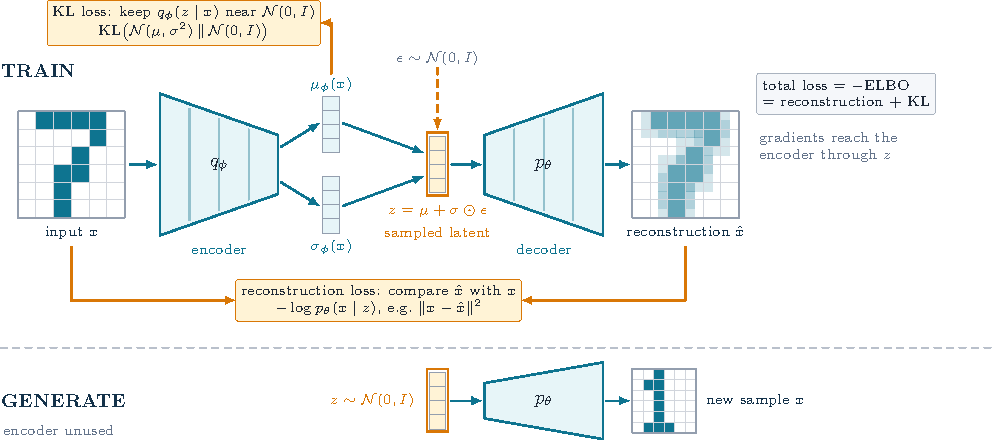
\includegraphics[width=0.95\textwidth]{vae_network.pdf}
  \vfill
  {\small 对角高斯时 $\KL(q\Vert p)=\tfrac12\sum_j(\mu_j^2+\sigma_j^2-\log\sigma_j^2-1)$ 有解析式；二值数据的重构项是逐位交叉熵，连续数据常用固定方差高斯，即 MSE。}
\end{frame}

\begin{frame}{重构与正则的拉锯}
  \begin{columns}[c]
    \begin{column}{0.52\textwidth}
      \centering
      \begin{tikzpicture}[x=1mm,y=1mm]
        \foreach \sx/\t/\c in {0/{KL 权重过小}/GRose,34/{KL 权重过大}/GRose}{%
          \draw[GSlate!50] (\sx,0) rectangle ++(28,28);
          \draw[GSlate!40,dashed] (\sx+14,14) circle (11);
          \node[lbl,anchor=north] at (\sx+14,-1) {\t};}
        \foreach \cx/\cy/\cc in {6/7/GTeal,21/8/GOrange,8/21/GNavy,22/21/GTeal!60}{%
          \foreach \dx/\dy in {0/0,1.2/0.6,-0.8/1,0.5/-1.1,-1/-0.6}{\fill[\cc] (\cx+\dx,\cy+\dy) circle (0.55);}}
        \foreach \dx/\dy/\cc in {0/0/GTeal,3/1/GOrange,-2/2/GNavy,1/-3/GTeal!60,-3/-2/GTeal,2/3/GOrange,4/-1/GNavy,-1/4/GTeal!60,-4/1/GOrange,0/-5/GNavy,5/2/GTeal,-2/-4/GOrange}{%
          \fill[\cc] (48+\dx,14+\dy) circle (0.55);}
      \end{tikzpicture}
      \par\vspace{1mm}
      {\scriptsize\slate{颜色表示不同类别样本的编码；虚线圈是先验 $\mathcal N(0,I)$ 的高概率区}}
    \end{column}
    \begin{column}{0.46\textwidth}
      \begin{itemize}
        \item KL 太弱：编码各自聚成小团，团间是空洞；从先验抽到空洞处，decoder 输出不像样
        \item KL 太强：所有编码都贴着先验，$z$ 不再携带样本信息，即 posterior collapse
        \item 高斯 decoder 相当于逐像素 MSE，对多种可能取平均，样本偏模糊
      \end{itemize}
    \end{column}
  \end{columns}
\end{frame}

\begin{frame}{VAE：小结}
  \centering
  \fourcard%
    {潜变量模型 $\int p(z)p_\theta(x\mid z)dz$\\encoder 近似后验}%
    {ELBO：重构 $-$ KL\\是 $\log p_\theta(x)$ 的下界}%
    {$z\sim p(z)$，一次 decoder\\再从 $p_\theta(x\mid z)$ 抽样}%
    {下界有间隙；样本偏模糊；posterior collapse}
  \vfill
  \begin{takeaway}
    VAE 用一个可优化的下界换掉难算的积分，并得到有意义的低维表示。今天的图像扩散模型常在 VAE 学出的潜空间里运行。
  \end{takeaway}
\end{frame}

% ====================================================================
\section{GAN：放弃似然}

\begin{frame}{生成器与判别器}
  \centering
  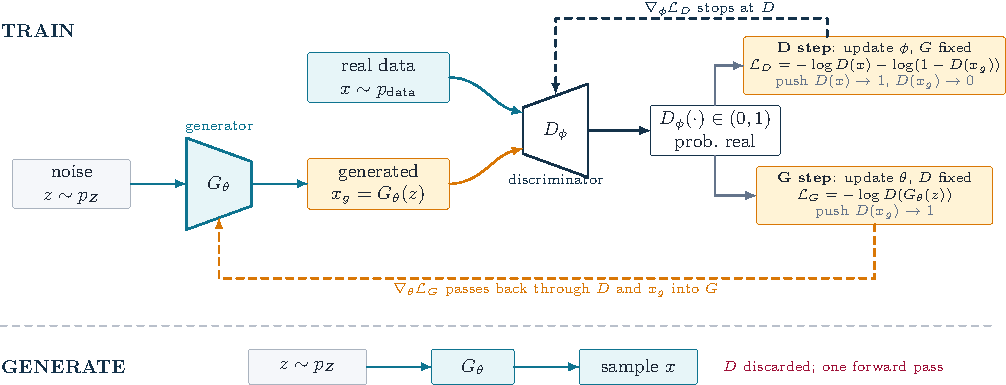
\includegraphics[width=0.95\textwidth]{gan_architecture.pdf}
  \vfill
  \begin{columns}[T]
    \begin{column}{0.48\textwidth}
      \small
      \textbf{训练}：两步交替。D step 固定 $G$，让真样本判 1、生成样本判 0；G step 固定 $D$，让 $D(G(z))$ 变大，梯度穿过 $D$ 回到 $G$。
    \end{column}
    \begin{column}{0.48\textwidth}
      \small
      \textbf{生成}：丢掉 $D$，$z$ 经 $G$ 一次前向就是样本。$D$ 只在训练中提供信号，整个模型不给出密度。
    \end{column}
  \end{columns}
\end{frame}

\begin{frame}{让一个分类器来当裁判}
  \begin{columns}[c]
    \begin{column}{0.5\textwidth}
      生成器 $G_\theta$：$z\sim\mathcal N(0,I)$ 一次前向得到 $x=G_\theta(z)$，不给密度。判别器 $D_\phi$ 判断样本来自数据还是生成器：
      \[
        \min_\theta\max_\phi\ \E_{p_{\mathrm{data}}}\log D+\E_{z}\log(1-D(G(z)))
      \]
      \begin{keystep}
        固定 $G$，最优判别器是密度比：
        \keyeq{D^*(x)=\frac{p_{\mathrm{data}}(x)}{p_{\mathrm{data}}(x)+p_g(x)}}
        代回后生成器在最小化 $2\,\mathrm{JSD}(p_{\mathrm{data}}\Vert p_g)-\log4$。
      \end{keystep}
    \end{column}
    \begin{column}{0.47\textwidth}
      \begin{tikzpicture}
        \begin{axis}[genai,width=7cm,height=4.4cm,xmin=-3.5,xmax=4,ymin=0,ymax=1.05,xtick=\empty,ytick={0,0.5,1},xlabel={$x$},domain=-3.5:4,legend style={at={(0.02,0.98)},anchor=north west}]
          \addplot[GOrange,fill=GAmber,fill opacity=0.6] {exp(-(x+0.5)^2/(2*0.64))/(0.8*sqrt(2*pi))} \closedcycle;
          \addlegendentry{$p_g$}
          \addplot[GTeal,fill=GSky,fill opacity=0.6] {exp(-(x-1.5)^2/(2*0.36))/(0.6*sqrt(2*pi))} \closedcycle;
          \addlegendentry{$p_{\mathrm{data}}$}
          \addplot[GNavy,dashed] {(exp(-(x-1.5)^2/(2*0.36))/0.6)/((exp(-(x-1.5)^2/(2*0.36))/0.6)+(exp(-(x+0.5)^2/(2*0.64))/0.8))};
          \addlegendentry{$D^*(x)$}
        \end{axis}
      \end{tikzpicture}
      \begin{concept}{两样本检验与似然比}
        判别器是一个学出来的检验统计量：它分不清两组样本，两个分布才相同。
      \end{concept}
    \end{column}
  \end{columns}
\end{frame}

\begin{frame}{GAN 的代价}
  \begin{columns}[T]
    \begin{column}{0.55\textwidth}
      \begin{itemize}
        \item 本讲唯一不以似然为目标的路线：没有密度，也报告不了样本的似然
        \item 训练是两个网络的博弈，交替更新不保证收敛；判别器过强时生成器梯度消失
        \item Mode collapse：生成器只覆盖少数容易骗过判别器的模式，行为接近第一讲的反向 KL
        \item 部署时一次前向，速度最快
      \end{itemize}
      \vspace{1mm}
      {\small\slate{另一种只用样本的办法：固定核函数，最小化两组样本的最大均值差异（MMD），不需要判别器。}}
    \end{column}
    \begin{column}{0.42\textwidth}
      \centering
      \begin{tikzpicture}[x=1mm,y=1mm]
        \pgfmathsetseed{9}
        \foreach \a in {0,45,...,315}{%
          \foreach \j in {1,...,7}{\fill[GTeal!70] ($(\a:15)+(1.6*rand,1.6*rand)$) circle (0.6);}}
        \foreach \a in {45,90}{%
          \foreach \j in {1,...,9}{\fill[GOrange] ($(\a:15)+(1.2*rand,1.2*rand)$) circle (0.6);}}
        \node[lblt,anchor=north] at (0,-19) {数据：8 个模式};
        \node[lblo,anchor=north] at (0,-23) {生成器：只覆盖 2 个};
      \end{tikzpicture}
    \end{column}
  \end{columns}
  \vfill
  \begin{takeaway}[小结]
    GAN 用一个可学习的检验统计量代替似然：采样最快、样本锐利，代价是无密度、训练不稳定、容易丢模式。
  \end{takeaway}
\end{frame}

% ====================================================================
\section{能量模型与 MCMC}

\begin{frame}{用神经网络参数化玻尔兹曼分布}
  \begin{columns}[c]
    \begin{column}{0.5\textwidth}
      \[
        p_\theta(x)=\frac{e^{-E_\theta(x)}}{Z_\theta},\qquad Z_\theta=\int e^{-E_\theta(x)}dx
      \]
      \begin{itemize}
        \item $E_\theta$ 可以是任意标量网络：表达最自由，不需要可逆，也不需要逐步分解
        \item 物理先验可以直接写进能量
        \item 代价全部落在 $Z_\theta$ 上：它同时出现在密度、采样和训练梯度中
      \end{itemize}
      \begin{concept}{玻尔兹曼分布}
        第一讲的形式，只是能量由数据学出来，温度并入 $E_\theta$。
      \end{concept}
    \end{column}
    \begin{column}{0.47\textwidth}
      \begin{tikzpicture}
        \begin{axis}[genai,width=7cm,height=5cm,xmin=-4,xmax=4.5,ymin=-0.05,ymax=1.15,xtick=\empty,ytick=\empty,xlabel={$x$},domain=-4:4.5,samples=241,legend style={at={(0.5,1.02)},anchor=south,legend columns=2}]
          \addplot[GNavy] {1-exp(-(x+2)^2/0.9)-0.9*exp(-(x-0.7)^2/0.8)-0.6*exp(-(x-3)^2/0.4)};
          \addlegendentry{$E_\theta(x)$}
          \addplot[GTeal,fill=GSky,fill opacity=0.7] {0.45*exp(-6*(1-exp(-(x+2)^2/0.9)-0.9*exp(-(x-0.7)^2/0.8)-0.6*exp(-(x-3)^2/0.4)))/exp(0)} \closedcycle;
          \addlegendentry{$\propto e^{-E_\theta}$}
        \end{axis}
      \end{tikzpicture}
    \end{column}
  \end{columns}
\end{frame}

\begin{frame}{似然梯度：正相位与负相位}
  \begin{columns}[T]
    \begin{column}{0.55\textwidth}
      \begin{keystep}
        $Z_\theta$ 算不出来，它的对数梯度却是一个期望：
        \keyeq{
          \nabla_\theta\log Z_\theta=\frac{1}{Z_\theta}\int-\nabla_\theta E_\theta\,e^{-E_\theta}dx=-\E_{p_\theta}[\nabla_\theta E_\theta]}
        于是负对数似然的梯度为
        \keyeq{
          \nabla_\theta\mathcal L
          =\underbrace{\E_{p_{\mathrm{data}}}[\nabla_\theta E_\theta]}_{\text{正相位}}
          -\underbrace{\E_{p_\theta}[\nabla_\theta E_\theta]}_{\text{负相位}}}
      \end{keystep}
      \begin{itemize}
        \item 正相位：压低数据处的能量
        \item 负相位：抬高模型样本处的能量，防止模型把所有能量都压低
      \end{itemize}
    \end{column}
    \begin{column}{0.42\textwidth}
      \begin{tikzpicture}
        \begin{axis}[genai,width=6.4cm,height=5cm,xmin=-4,xmax=4.5,ymin=-0.2,ymax=1.3,xtick=\empty,ytick=\empty,xlabel={$x$},domain=-4:4.5,samples=241]
          \addplot[GNavy] {1-exp(-(x+2)^2/0.9)-0.9*exp(-(x-0.7)^2/0.8)-0.6*exp(-(x-3)^2/0.4)};
          \addplot[only marks,mark=*,mark size=1.6pt,GTeal] coordinates {(-2.2,-0.1)(-1.9,-0.1)(-2.0,-0.1)(0.5,-0.1)(0.7,-0.1)};
          \addplot[only marks,mark=*,mark size=1.6pt,GOrange] coordinates {(2.9,-0.1)(3.1,-0.1)(-2.1,-0.1)};
          \draw[-{Latex[length=1.6mm]},GTeal,line width=1pt] (axis cs:-2,0.35) -- (axis cs:-2,0.08);
          \draw[-{Latex[length=1.6mm]},GTeal,line width=1pt] (axis cs:0.6,0.45) -- (axis cs:0.6,0.18);
          \draw[-{Latex[length=1.6mm]},GOrange,line width=1pt] (axis cs:3,0.45) -- (axis cs:3,0.8);
          \node[font=\scriptsize,text=GTeal] at (axis cs:-1.2,1.15) {数据：压低};
          \node[font=\scriptsize,text=GOrange] at (axis cs:2.6,1.15) {模型样本：抬高};
        \end{axis}
      \end{tikzpicture}
      \par\vspace{1mm}
      {\scriptsize\slate{两项平衡时，模型样本与数据分布一致。每一步更新前都要先从当前模型采样。}}
    \end{column}
  \end{columns}
\end{frame}

\begin{frame}{马尔可夫链蒙特卡洛}
  \begin{columns}[T]
    \begin{column}{0.55\textwidth}
      构造一条马尔可夫链 $x_0\to x_1\to\cdots$，使目标 $\pi$ 是它的平稳分布；跑得足够久，状态就近似服从 $\pi$。
      \begin{keystep}[细致平衡]
        若转移核满足 $\pi(x)K(x'\mid x)=\pi(x')K(x\mid x')$，对 $x$ 求和即得
        $\sum_x\pi(x)K(x'\mid x)=\pi(x')$，$\pi$ 是平稳分布。
      \end{keystep}
      \textbf{Metropolis--Hastings}：从 $q(x'\mid x)$ 提议，以
      \[
        a=\min\Bigl\{1,\ \frac{\tilde\pi(x')\,q(x\mid x')}{\tilde\pi(x)\,q(x'\mid x)}\Bigr\}
      \]
      接受，否则留在原地。只用到比值，$Z$ 被约掉。
    \end{column}
    \begin{column}{0.42\textwidth}
      \centering
      \begin{tikzpicture}[x=1mm,y=1mm]
        \foreach \r/\o in {3/0.9,6/0.6,9/0.35}{%
          \draw[GTeal,opacity=\o,rotate around={30:(14,20)}] (14,20) ellipse ({\r*1.3} and {\r*0.8});
          \draw[GTeal,opacity=\o] (42,12) ellipse ({\r} and {\r*0.9});}
        \draw[GNavy,line width=0.6pt] (6,16) -- (9,19) -- (12,17) -- (15,22) -- (13,24) -- (17,21) -- (19,24) -- (16,19) -- (20,18) -- (23,22) -- (21,25) -- (18,23);
        \foreach \p in {(6,16),(9,19),(12,17),(15,22),(13,24),(17,21),(19,24),(16,19),(20,18),(23,22),(21,25),(18,23)}{\fill[GNavy] \p circle (0.6);}
        \foreach \p in {(28,14),(4,28),(25,8)}{\node[GRose,font=\scriptsize] at \p {$\times$};}
        \draw[GRose,dashed] (20,18) -- (28,14);
        \draw[GRose,dashed] (13,24) -- (4,28);
        \node[lbl,anchor=north,text width=55mm] at (24,4) {链在一个模式内游走；$\times$ 是被拒绝的提议。另一模式很难到达};
      \end{tikzpicture}
      \begin{concept}{马尔可夫链与平稳分布}
        遍历性保证极限存在；收敛快慢由混合时间决定。
      \end{concept}
    \end{column}
  \end{columns}
\end{frame}

\begin{frame}{Langevin 动力学：沿梯度下坡，再加热噪声}
  \begin{columns}[T]
    \begin{column}{0.5\textwidth}
      连续变量时，用能量梯度构造提议：
      \[
        x_{k+1}=x_k-\tfrac{\eta}{2}\nabla_xE(x_k)+\sqrt{\eta}\,\xi_k
      \]
      \begin{itemize}
        \item 下坡项推向低能区，噪声 $\xi_k\sim\mathcal N(0,I)$ 让样本有机会翻越势垒
        \item 连续极限以 $e^{-E}$ 为平稳分布；有限步长的偏差可用 MH 校正
        \item 混合慢：势垒高时，链要很久才跨到另一个谷
      \end{itemize}
      \begin{concept}{布朗运动}
        $dx=-\tfrac12\nabla E\,dt+dW_t$；第三讲的扩散模型用同一类随机微分方程。
      \end{concept}
    \end{column}
    \begin{column}{0.48\textwidth}
      \begin{tikzpicture}
        \begin{axis}[genai,width=7.2cm,height=4.6cm,xmin=0,xmax=24,ymin=-1.9,ymax=1.9,xlabel={步数 $k$},ylabel={$x_k$},ytick={-1,0,1},xtick={0,10,20},xticklabels={0,1000,2000}]
          \draw[GSlate!40,dashed,line width=0.5pt] (axis cs:0,1) -- (axis cs:24,1);
          \draw[GSlate!40,dashed,line width=0.5pt] (axis cs:0,-1) -- (axis cs:24,-1);
          \addplot[GTeal,line width=0.6pt] table[x expr=\thisrow{k}/100,y=x] {../shared/figures/langevin_path.dat};
        \end{axis}
      \end{tikzpicture}
      \par{\scriptsize\slate{双势阱 $E=(x^2-1)^2/T$ 中的一条 Langevin 链：长时间停在一个谷里，偶尔跃迁}}
    \end{column}
  \end{columns}
\end{frame}

\begin{frame}{训练能量模型的实际做法}
  \begin{columns}[T]
    \begin{column}{0.5\textwidth}
      每次参数更新都要负相位样本，而充分混合的链太贵。常用有偏但便宜的近似：
      \begin{itemize}
        \item \textbf{CD-$k$}：从数据点出发只跑 $k$ 步，用短链终点作负样本；只修正数据附近的错误
        \item \textbf{持续链}：保存上一轮的链状态，下一轮接着跑；不必每次重新预热，但参数在变，链在追一个移动的目标
      \end{itemize}
      推理时同样要跑链：生成一个样本需要成百上千步。
    \end{column}
    \begin{column}{0.47\textwidth}
      \fourstack{$p_\theta\propto e^{-E_\theta}$\\最灵活，未归一化}{正相位 $-$ 负相位\\（极大似然的梯度）}{MCMC / Langevin\\多步迭代}{负相位昂贵；混合慢；样本有偏}
    \end{column}
  \end{columns}
\end{frame}

\begin{frame}{Score：一个与 $Z$ 无关的量}
  \begin{columns}[c]
    \begin{column}{0.5\textwidth}
      \[
        s(x)=\nabla_x\log p(x)=-\nabla_xE(x)
      \]
      $Z$ 对 $x$ 是常数，求梯度后消失。score 是指向密度上升最快方向的向量场。
      \begin{keystep}[score matching]
        用 Fisher 散度比较两个分布：$D_F(p\Vert q)=\tfrac12\E_p\|\nabla\log p-\nabla\log q\|^2$，它只看两者的 score 是否处处一致。取 $q=p_\theta$，分部积分去掉未知的 $\nabla\log p_{\mathrm{data}}$：
        \keyeq{
          D_F(p_{\mathrm{data}}\Vert p_\theta)
          =\E_{p_{\mathrm{data}}}\Bigl[\tfrac12\|s_\theta\|^2+\nabla\cdot s_\theta\Bigr]+C}
        只用数据样本，不需要负样本。
      \end{keystep}
    \end{column}
    \begin{column}{0.47\textwidth}
      \centering
      \begin{tikzpicture}[x=9mm,y=9mm]
        \foreach \r/\o in {0.35/0.9,0.7/0.6,1.05/0.35}{%
          \draw[GTeal,opacity=\o] (-1.6,-0.4) circle (\r);
          \draw[GTeal,opacity=\o] (1.5,0.6) circle (\r);}
        \input{figures/score_field.tex}
        \fill[GTeal] (-1.6,-0.4) circle (0.06);
        \fill[GTeal] (1.5,0.6) circle (0.06);
      \end{tikzpicture}
      \par\vspace{1mm}
      {\scriptsize\slate{双峰分布的 score 场：箭头指向附近的模式}}
    \end{column}
  \end{columns}
\end{frame}

% ====================================================================
\begin{frame}{第二讲小结}
  \small
  \renewcommand{\arraystretch}{1.15}
  \begin{tabularx}{\textwidth}{@{}>{\leavevmode\color{GNavy}\bfseries}p{16mm} >{\raggedright\arraybackslash}p{30mm} >{\raggedright\arraybackslash}p{28mm} >{\raggedright\arraybackslash}p{22mm} >{\raggedright\arraybackslash}X@{}}
    \toprule
    & 概率对象 & 训练目标 & 采样 & 主要代价\\
    \midrule
    自回归 & $\prod_tp(x_t\mid x_{<t})$ & 极大似然（交叉熵） & 逐个抽样 & 串行\\
    Flow & 可逆变换 + Jacobian & 精确极大似然 & 逆变换一次 & 结构受限\\
    VAE & 潜变量的连续混合 & ELBO（下界） & decoder 一次 & 下界间隙、模糊\\
    GAN & 隐式分布 & 对抗博弈（JSD） & 生成器一次 & 无密度、丢模式\\
    能量模型 & $e^{-E_\theta}/Z_\theta$ & 正相位 $-$ 负相位 & MCMC 多步 & 混合慢\\
    \bottomrule
  \end{tabularx}
  \vspace{3mm}
  \begin{takeaway}
    每一类模型都在“能否算出 $p(x)$”与“采样是否便宜”之间取舍。能量模型最灵活，却被采样拖累；score 绕开了 $Z$，但学到 score 之后怎样高效采样？如果在不同噪声水平上都学一个 score，会发生什么？这就是第三讲的扩散模型。
  \end{takeaway}
\end{frame}

\end{document}
